\chapter{إجراءات التشغيل القياسية}
\label{ch:02-sops}

\section{ما إجراء التشغيل القياسي؟}
\label{sec:sops-what}

إجراء التشغيل القياسي طريقة متفق عليها لأداء عمل يتكرر: ما الذي يبدؤه، ومن يؤدي كل خطوة، ومن يقرر، وما النتيجة التي تُحفظ. وحين يُكتب الإجراء على ورق يبقى تطبيقه رهيناً بذاكرة الناس؛ أما في كيان فيصبح مساراً يعرض على كل شخص خطوته في وقتها، ويحفظ كل قرار مع صاحبه وتاريخه.

\begin{rcnote}[مثال: مديرية الواحة]
مسار الكشف في الفصل الأول إجراء تشغيل قياسي: يبدأ بتكليف من خالد، وتؤدي ليلى خطوات الكشف، وتقرر رنا، ثم يُحفظ القرار في الكشف وسجل «فرن السنابل».
\end{rcnote}

\begin{table}[H]
\centering
\caption{أجزاء الإجراء}
\label{tab:sops-parts}
\begin{tabularx}{\linewidth}{R{3.6cm} Y}
\rcHeaderRow
\thh{الجزء} & \thh{السؤال الذي يجيب عنه}\\
البداية & ما الحدث الذي يبدأ الإجراء؟ كإرسال نموذج أو إنشاء سجل.\\
الخطوات & من يؤدي كل خطوة، وبأي ترتيب؟\\
القرار & من يقرر، وما الخيارات المتاحة له؟ ويُكتب سبب الإعادة أو الرفض ليفهمه من يتابع.\\
النتيجة & ما الذي يتغير بعد كل قرار؟ كتحديث سجل أو إنشاء مهمة أو إغلاق الطلب.\\
الأثر & أين تجد لاحقاً ما حدث ومن قرّره ومتى؟\\
\end{tabularx}
\end{table}

\begin{figure}[H]
\centering
\begin{tikzpicture}[node distance=0.5cm]
\node[stepBox] (a) {\RL{حدث يبدأ الإجراء}};
\node[stepBox,below=of a] (b) {\RL{خطوات يؤديها أشخاص}};
\node[stepBox,below=of b] (c) {\RL{قرار المراجِع}};
\node[stepBox,below=of c] (d) {\RL{نتيجة تُحفظ\\مع صاحب القرار وتاريخه}};
\draw[flowsTo] (a) -- (b);
\draw[flowsTo] (b) -- (c);
\draw[flowsTo] (c) -- (d);
\end{tikzpicture}
\rclegend
\caption{شكل إجراء فيه قرار مراجعة}
\label{fig:sops-shape}
\shotnote{يبيّن المخطط أن الإجراء لا ينتهي بأداء الخطوات، بل بقرار يتخذه مراجِع ثم بنتيجة محفوظة يمكن الرجوع إليها. ويختلف أثر القرار بحسب نوعه، كما يبيّن الجدول التالي؛ لذلك صمّم أثر كل قرار وجرّبه، لا الاعتماد وحده.}
\end{figure}

\begin{table}[H]
\centering
\caption{ماذا يحدث بعد كل قرار؟}
\label{tab:sops-decisions}
\begin{tabularx}{\linewidth}{R{3.6cm} Y}
\rcHeaderRow
\thh{القرار} & \thh{أثره}\\
اعتماد & تُحفظ النتيجة، وتُحدَّث السجلات المرتبطة إن صُمّم الإجراء لذلك.\\
إعادة للتصحيح & يعود العمل إلى من أعدّه مع ملاحظات المراجِع، فيعدّله ويرسله من جديد، وتبدأ جولة مراجعة أخرى.\\
رفض & يُغلق العمل مع سبب الرفض، ولا تتغير السجلات المرتبطة.\\
\end{tabularx}
\end{table}

\section{اختر الأداة التي تنفذ الإجراء}
\label{sec:sops-tools}

لا تبدأ بالأداة، بل بكتابة الإجراء بلغة العمل. فإذا عرفت أجزاءه، اختر من أدوات البناء الأداة التي تنفذه. وتختار بينها بحسب مكان العمل: داخل نموذج واحد، أو بين أشخاص وسجلات داخل التطبيق، أو بحدث يتطلب أتمتة.

\begin{rcnote}[مثال: مديرية الواحة]
يمر كشف «فرن السنابل» بحالات وينتهي بقرار مدقق، لذلك تبدأ المديرية بمسار الطلب في نموذج الكشف. وإذا أرادت لاحقاً أن تُنشأ مهمة متابعة لخالد بعد كل رفض، أضافت إجراءً داخلياً لهذه الخطوة.
\end{rcnote}

\begin{table}[H]
\centering
\caption{أي أداة تختار؟}
\label{tab:sops-tools}
\begin{tabularx}{\linewidth}{R{3.6cm} Y}
\rcHeaderRow
\thh{الأداة} & \thh{متى تختارها؟ ومن أين تبدأ؟}\\
مسار الطلب في النموذج & عندما يمر الرد على نموذج واحد بحالات وموافقات يراها مقدّمه. تبدأ من «منشئ النماذج» ← «المسار» ← «تفعيل المسار».\\
«الإجراءات الداخلية» & عندما يحتاج العمل إلى خطوات متتابعة داخل التطبيق، مثل «طلب موافقة» ثم «إنشاء مهمة» أو تحديث سجل أو إرسال إشعار. تبدأ من «ادوات البناء» ← «الأساسية» ← «الإجراءات الداخلية».\\
«إجراءات التشغيل القياسية» & عندما يبدأ العمل بحدث وتريد أن تتحقق الأتمتة من البيانات ثم تنفذ إجراءً تلقائياً، كإنشاء مهمة أو إرسال إشعار. تبدأ من «ادوات البناء» ← «الأساسية» ← «إجراءات التشغيل القياسية».\\
\end{tabularx}
\end{table}

\begin{figure}[H]
\centering
\begin{tikzpicture}[node distance=0.5cm]
\node[stepBox] (a) {\RL{هل يدور العمل حول\\ردّ على نموذج واحد؟}};
\node[stepBox,below=of a] (b) {\RL{نعم: ابدأ بمسار الطلب}};
\node[stepBox,below=of b] (c) {\RL{هل يحتاج بعد القرار\\إلى مهام أو سجلات أخرى؟}};
\node[stepBox,below=of c] (d) {\RL{نعم: أضف إجراءً داخلياً\\لهذه الخطوات}};
\draw[flowsTo] (a) -- (b);
\draw[flowsTo] (b) -- (c);
\draw[flowsTo] (c) -- (d);
\end{tikzpicture}
\rclegend
\caption{ترتيب الاختيار بين الأدوات}
\label{fig:sops-choose}
\shotnote{يقترح المخطط أن تبدأ بأبسط أداة تكفي العمل، ثم تضيف أداة أخرى للخطوات التي لا تغطيها. فمسار الطلب يكفي ما دام القرار يخص الرد نفسه؛ أما إنشاء مهام أو تحديث سجلات أخرى بعد القرار فيحتاج إلى إجراء داخلي.}
\end{figure}

ويفصّل الفصل \ref{ch:03-compare} الفرق بين هذه الأدوات، ويضيف إليها «دليل الإجراءات» وحزم النماذج.

\section{اكتب الإجراء قبل أن تبنيه}
\label{sec:sops-write}

يكشف الإجراء المكتوب ما ينقص قبل أن يظهر في التشغيل: خطوة بلا مسؤول، أو قرار لا يُعرف أثره، أو منشأة تتغير بياناتها قبل المراجعة. لذلك اكتب أجزاءه الخمسة في جدول واحد، واعرضه على من سيعملون به.

\begin{rcnote}[مثال: مديرية الواحة]
كتبت المديرية إجراء تدقيق الكشف قبل بنائه، وراجعته مع خالد وليلى ورنا حتى عرف كل منهم خطوته. ويعرض الجدول التالي ما كتبته.
\end{rcnote}

\begin{table}[H]
\centering
\caption{مثال: إجراء تدقيق الكشف في مديرية الواحة}
\label{tab:sops-example}
\begin{tabularx}{\linewidth}{R{3.6cm} Y}
\rcHeaderRow
\thh{الجزء} & \thh{ما كتبته المديرية}\\
البداية & ترسل ليلى كشف «فرن السنابل» بعد الزيارة.\\
الخطوات & يصبح الكشف «قيد التدقيق»، فيتوقف تعديل ليلى، ويصل إلى رنا.\\
القرار & تعتمد رنا الكشف، أو تعيده مع ما يحتاج تصحيحاً، أو ترفضه مع السبب.\\
النتيجة & بعد الاعتماد يُحدَّث عنوان الفرن وحالة توثيقه؛ وبعد الرفض يبقى الفرن دون تغيير.\\
الأثر & يبقى القرار وصاحبه وتاريخه في الكشف، ومرجع الكشف المعتمد في سجل الفرن.\\
\end{tabularx}
\end{table}

\subsection{خطوات العمل والتحقق}
\begin{enumerate}
\item اكتب اسم الإجراء والنتيجة التي يجب أن يصل إليها.
\item حدّد الحدث الذي يبدؤه، واكتب الخطوات بالترتيب مع اسم المسؤول عن كل خطوة.
\item حدّد من يقرر وما خياراته، واكتب ما يحدث بعد كل خيار، بما في ذلك سبب الإعادة أو الرفض.
\item اختر الأداة من جدول «أي أداة تختار؟»، ثم ابنِ الإجراء.
\item جرّب أثر كل قرار بسجل تجريبي قبل أن يستخدم الفريق الإجراء.
\end{enumerate}

\textbf{تحقق:} اسأل كل من سيعمل بالإجراء عن خطوته وما يحدث بعد قراره. فإذا لم يجد أحدهم جواباً واضحاً، أكمل الإجراء المكتوب قبل البناء؛ لأن الأداة تنفذ ما صممته، ولا تسد نقصاً في الإجراء.

\section{ابنِ الإجراء بمسار الطلب في النموذج}
\label{sec:sops-journey}

مسار الطلب يرسم ما يحدث للرد بعد إرساله: الحالات التي يمر بها، والموافقات التي تجري في الطريق، ومن يرى كل مرحلة. وتعدّه من مكان واحد داخل النموذج، ولا يتغير شيء على الفريق حتى تنشر النموذج.

\begin{rcnote}[مثال: مديرية الواحة]
يضيف مسؤول النظام إلى نموذج الكشف الحالات «قيد التدقيق» و«مقبول» و«مرفوض» و«بحاجة إلى تصحيح»، ثم «خطوة موافقة» تراجع فيها رنا يوسف كل كشف يصل إلى «قيد التدقيق».
\end{rcnote}

\begin{figure}[H]
\centering
\begin{tikzpicture}[node distance=0.5cm]
\node[stepBox] (a) {\RL{تفعيل المسار}};
\node[stepBox,below=of a] (b) {\RL{إضافة الحالات}};
\node[stepBox,below=of b] (c) {\RL{خطوة موافقة\\ومن يراجع فيها}};
\node[stepBox,below=of c] (d) {\RL{اختبار النموذج ونشره}};
\draw[flowsTo] (a) -- (b);
\draw[flowsTo] (b) -- (c);
\draw[flowsTo] (c) -- (d);
\end{tikzpicture}
\rclegend
\caption{ترتيب إعداد مسار الطلب}
\label{fig:sops-journey-order}
\shotnote{يرتب المخطط الإعداد كما يعتمد بعضه على بعض: فخطوة الموافقة تعمل في حالات محددة، لذلك تُضاف الحالات قبلها. وينتهي الإعداد بالاختبار ثم النشر، لأن الفريق لا يرى أي تعديل قبل النشر.}
\end{figure}

\begin{table}[H]
\centering
\caption{ما الذي تضبطه في المسار؟}
\label{tab:sops-journey-parts}
\begin{tabularx}{\linewidth}{R{3.6cm} Y}
\rcHeaderRow
\thh{الجزء} & \thh{ما يضبطه}\\
«الحالات» & الحالات التي يمر بها الرد، مثل حالة التدقيق والحالتين النهائيتين.\\
«خطوة موافقة» & من يراجع، وفي أي حالة تبدأ المراجعة، وإلى أي حالة ينتقل الرد بعد القرار.\\
الإعادة للتصحيح & يؤشر المراجِع على الإجابات التي «يحتاج تصحيحًا» ويطلب التعديلات؛ وعندما يرسل مقدّم الطلب الرد بعد تعديله تبدأ جولة موافقة جديدة.\\
\end{tabularx}
\end{table}

\subsection{خطوات العمل والتحقق}
\begin{enumerate}
\item افتح النموذج في «منشئ النماذج»، ثم «المسار»، واضغط «تفعيل المسار».
\item أضف في «الحالات» حالة للتدقيق وحالتين للقبول والرفض.
\item أضف «خطوة موافقة»، واختر المراجِع، واجعلها تبدأ في حالة التدقيق.
\item جرّب النموذج بحساب مُعِدّ وحساب مراجِع، ثم انشره.
\end{enumerate}

\textbf{تحقق:} أرسل رداً تجريبياً؛ يجب أن ينتقل إلى حالة التدقيق ويظهر طلب الموافقة عند المراجِع. وإذا لم يظهر، فتأكد من أن الحالة التي انتقل إليها الرد هي نفسها التي تبدأ فيها خطوة الموافقة.

\begin{figure}[H]
\centering
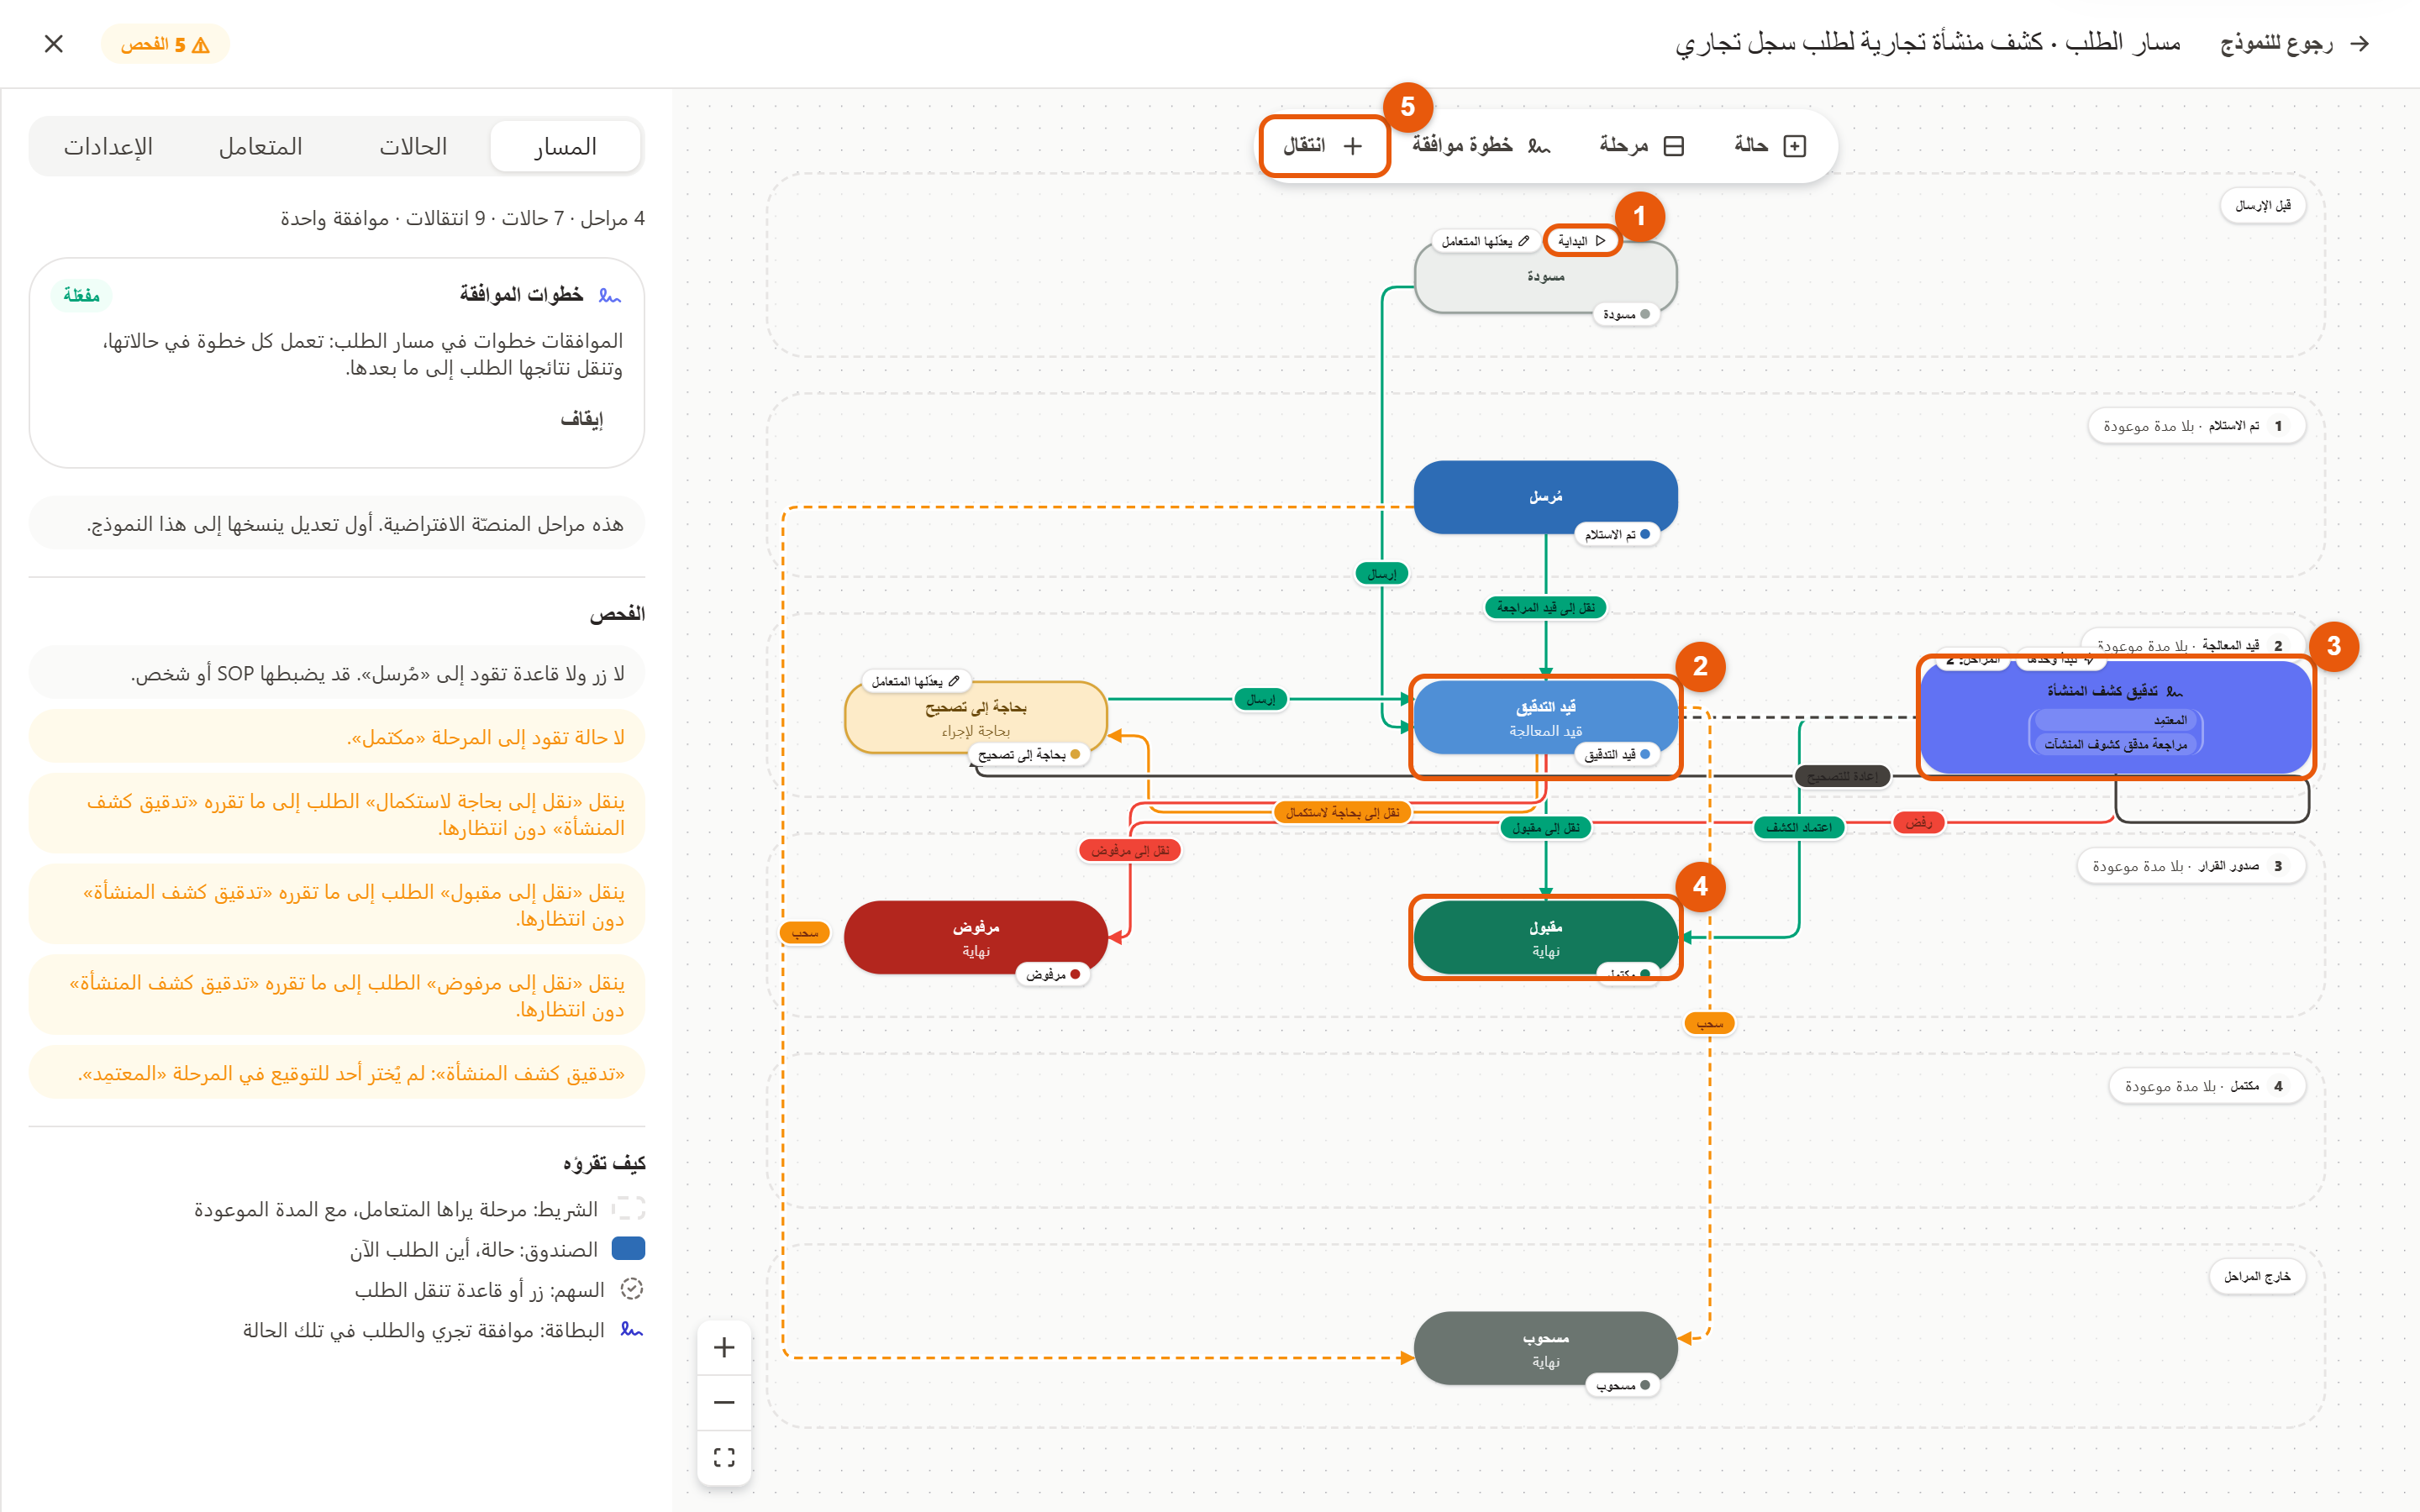
\includegraphics[width=0.95\linewidth]{assets/screens/journey-map.png}
\caption{خريطة مسار الطلب}
\label{fig:sops-journey-map}
\shotnote{تعرض الخريطة كل حالة في صندوق، وكل انتقال في سهم، وكل موافقة في بطاقة. وتلخّص اللوحة الجانبية ما فيها وتعرض «الفحص». ① «البداية»: الحالة التي يبدأ منها الرد. ② «قيد التدقيق»: الحالة التي تبدأ فيها الموافقة. ③ خطوة الموافقة: تحدد المراجِع وتقرر الانتقال التالي. ④ «مقبول»: نهاية المسار الناجحة. ⑤ «حالة» و«مرحلة» و«خطوة موافقة» و«انتقال»: أزرار إضافة عناصر المسار.}
\end{figure}

\subsection{افحص المسار قبل النشر}

يراجع «الفحص» المسار كله، وينبهك إلى ما سيعطّله أو يتجاوز المراجعة. لذلك افتحه بعد كل تعديل، ولا تكتفِ بنجاح رد تجريبي واحد.

\begin{figure}[H]
\centering
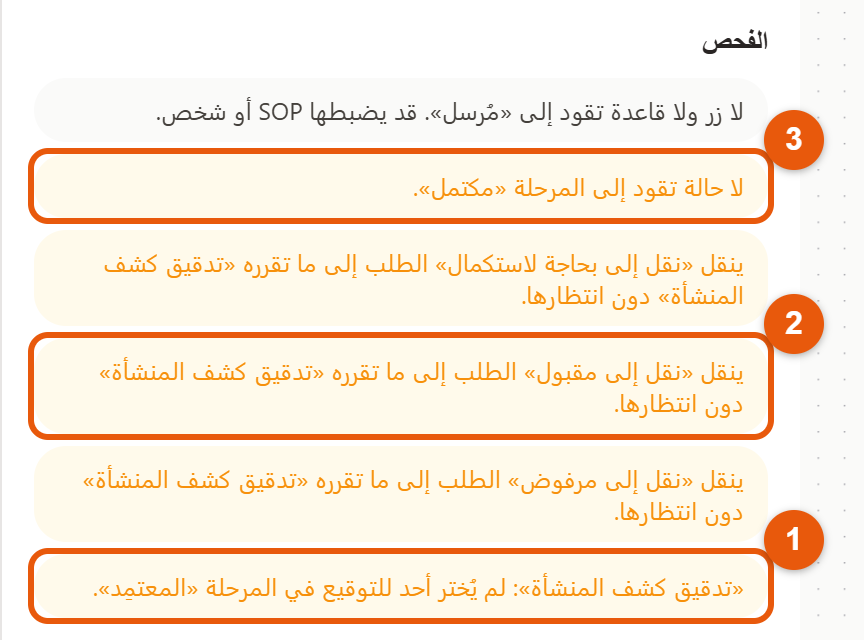
\includegraphics[width=0.9\linewidth]{assets/screens/journey-check.png}
\caption{تنبيهات «الفحص»}
\label{fig:sops-journey-check}
\shotnote{تعرض الصورة مساراً لم يكتمل بعد، وتتكرر فيه تنبيهات شائعة. ويشرح الجدول التالي معالجة كل منها. ① خطوة موافقة بلا موقّع: لن يستطيع أحد إنهاءها. ② زر ينقل الطلب دون انتظار الموافقة: يتجاوز المدقق. ③ مرحلة لا تصل إليها أي حالة: لن يراها المتعامل مكتملة.}
\end{figure}

\begin{table}[H]
\centering
\caption{كيف تعالج تنبيهات «الفحص»؟}
\label{tab:sops-journey-check}
\begin{tabularx}{\linewidth}{R{5.4cm} Y}
\rcHeaderRow
\thh{التنبيه} & \thh{المعالجة}\\
«لم يُختر أحد للتوقيع في المرحلة» & افتح خطوة الموافقة، واختر المراجِع. وعالج هذا أولاً، لأن الكشف سيتوقف عنده.\\
«ينقل … الطلب إلى ما تقرره … دون انتظارها» & أزل زر النقل أو أخفِه، واترك الانتقال لنتائج خطوة الموافقة.\\
«لا زر ولا قاعدة تقود إلى» حالة & أضف انتقالاً إليها، أو احذفها إذا لم تعد تحتاج إليها.\\
«لا حالة تقود إلى المرحلة» & اربط حالة النهاية الناجحة بتلك المرحلة، حتى يرى المتعامل اكتمال طلبه.\\
\end{tabularx}
\end{table}

\begin{rcnote}[مثال: مديرية الواحة]
أضافت المديرية أزراراً لنقل الكشف مباشرة، فنبّهها «الفحص» إلى أنها تتجاوز موافقة رنا. فأزالتها، وأصبح الانتقال إلى «مقبول» أو «مرفوض» نتيجة لقرار رنا فقط.
\end{rcnote}

\section{تابع الإجراء بعد التشغيل}
\label{sec:sops-follow}

بعد النشر يبدأ الإجراء العمل على ردود حقيقية، ويحتاج إلى متابعة: ما الذي ينتظر، ومن تأخر، وما الذي فشل. ولكل أداة مكان تتابع فيه عملها.

\begin{table}[H]
\centering
\caption{أين تتابع الإجراء؟}
\label{tab:sops-follow}
\begin{tabularx}{\linewidth}{R{3.6cm} Y}
\rcHeaderRow
\thh{الأداة} & \thh{مكان المتابعة}\\
مسار الطلب في النموذج & صفحة «العمل» في النموذج: ما يجري في التعبئة والموافقات، وما ينتظر في كل مرحلة وما تأخر.\\
«الإجراءات الداخلية» & «عمليات التشغيل»: حالة كل تشغيل ونتيجته، وإعادة التشغيل الفاشل.\\
المراجِع & «طلبات بانتظارك»: الموافقات التي تنتظر رده.\\
\end{tabularx}
\end{table}

\begin{rcnote}[مثال: مديرية الواحة]
يفتح خالد صفحة «العمل» في نموذج الكشف كل صباح، فيرى عدد الكشوف التي تنتظر رنا، والكشف الذي أُعيد إلى ليلى ولم ترسله بعد.
\end{rcnote}

\begin{rcchecklist}[قائمة تحقق: إجراء جاهز للتشغيل]
\begin{checklist}
  \item للإجراء بداية واحدة واضحة، ولكل خطوة مسؤول معروف.
  \item المراجِع شخص غير من أعدّ العمل.
  \item جُرّب أثر الاعتماد والإعادة والرفض بسجل تجريبي.
  \item يعرف المسؤول أين يتابع ما ينتظر وما تأخر.
\end{checklist}
\end{rcchecklist}
